\section*{Entreprise}
%\addcontentsline{toc}{section}{Entreprise} 

\subsection*{Groupe BPCE}
%\addcontentsline{toc}{subsection}{Groupe BPCE} 
Au terme d’un rapprochement entamé en 2006, les réseaux Banque Populaire et Caisse d’Epargne fusionnent leurs organes centraux le 31 juillet 2009. Le Groupe BPCE, deuxième groupe bancaire en France, est né.
\\
\\
Le Groupe BPCE est présent dans la banque de proximité et l’assurance en France grâce à la coopeération Banque Populaire et Caisse d’Epargne. Il déploie également au niveau mondial les métiers de gestion d’actifs et de fortune, avec Natixis Investment Managers, et de banque de grande clientèle avec Natixis Corporate \& Investment Banking.
\\
\\
Dans le fonctionnement du Groupe, les sociétaires sont le socle du modèle. Ils sont les propriétaires de 100\% du capital des Banques Populaires et des Caisses d’Epargne au travers de parts sociales. Leurs représentants constituent les conseils d’administration des Banques Populaires et les conseils d’orientation et de surveillance des Caisses d’Epargne.
\\
Les Banques Populaires et les Caisses d’Epargne détiennent à parité 100\% du capital de BPCE qui est l'organe central du Groupe. Enfin l'on retrouve les filiales de BPCE dont Natixis, la Banque Palatine, Oney et les filiales regroupées dans le pôle Solutions et Expertises financières.        


\begin{figure}[h!]
  \caption{Titre de la figure (source : \cite{ahu61})}
  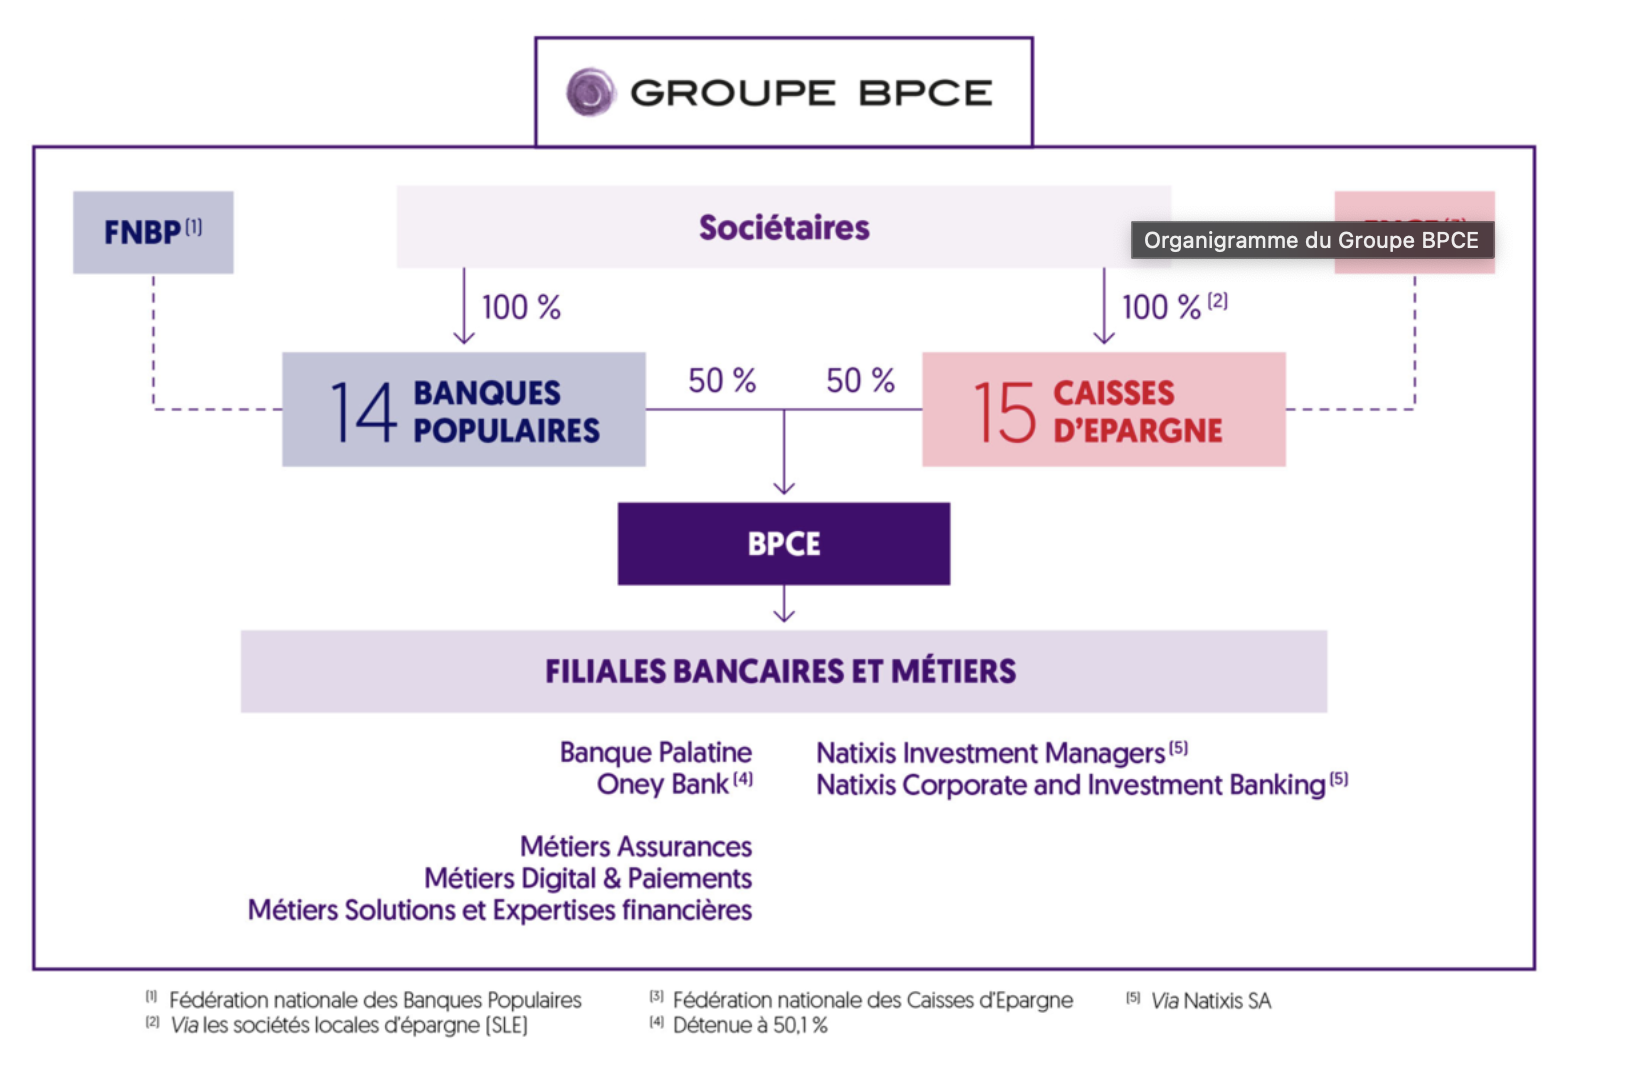
\includegraphics[width=\linewidth]{./img/intro/bpce_orga}
\end{figure}


\subsection*{Natixis Investment Managers}
%\addcontentsline{toc}{subsection}{Natixis Investment Managers} 
Natixis Investment Managers se fonde sur la force d’une approche indépendante en matière de gestion d’actifs. Chaque société de gestion affilée se concentre sur les styles et disciplines d'investissement pour lesquels elle dispose d'une expertise éprouvée. Il en résulte une sélection de plus de 200 stratégies d’investissement élaborées par des sociétés de gestion dont certaines figurent parmi les plus réputées au monde.

\begin{figure}[h!]
  \caption{Titre de la figure (source : \cite{ab94})}
  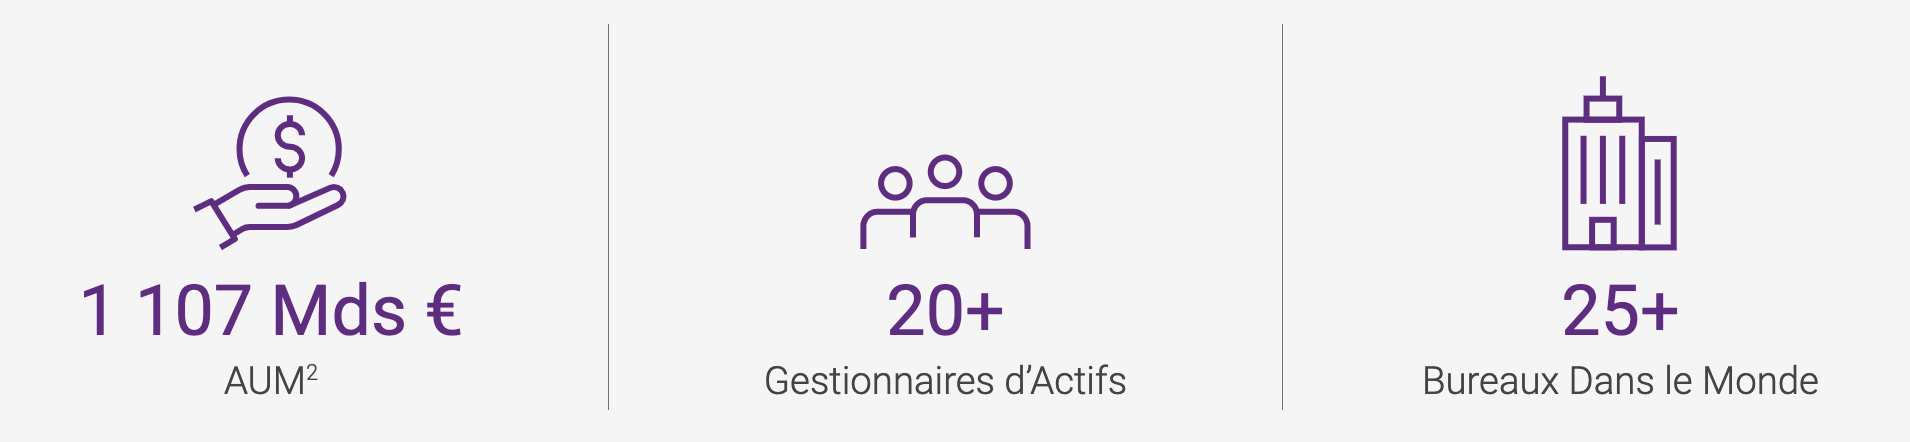
\includegraphics[width=\linewidth]{./img/intro/nim_kpi}
\end{figure}


\begin{figure}[h!]
  \caption{Titre de la figure (source : \cite{m85})}
  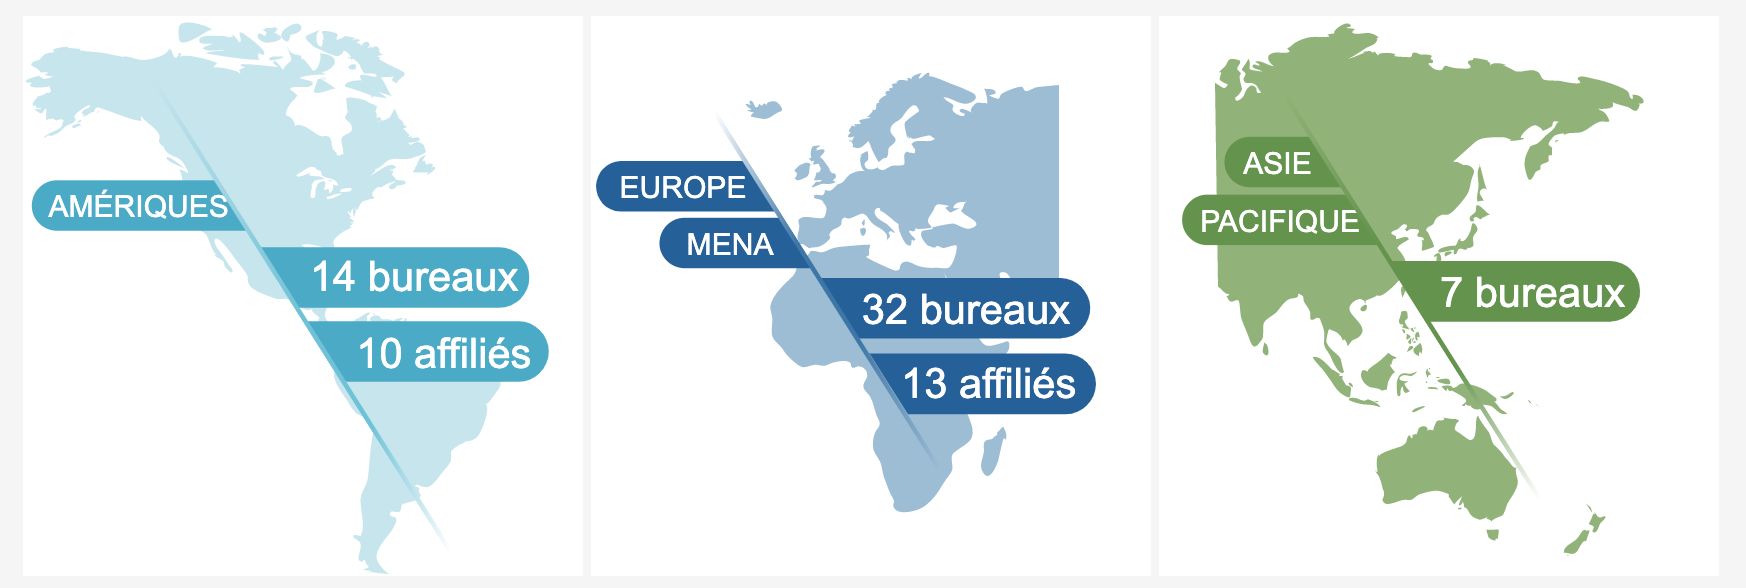
\includegraphics[width=\linewidth]{./img/intro/nim_loc}
\end{figure}



\subsection*{Seeyond}
%\addcontentsline{toc}{subsection}{Seeyond} 


\begin{figure}[h!]
  \caption{Titre de la figure (source : \cite{ah2006})}
  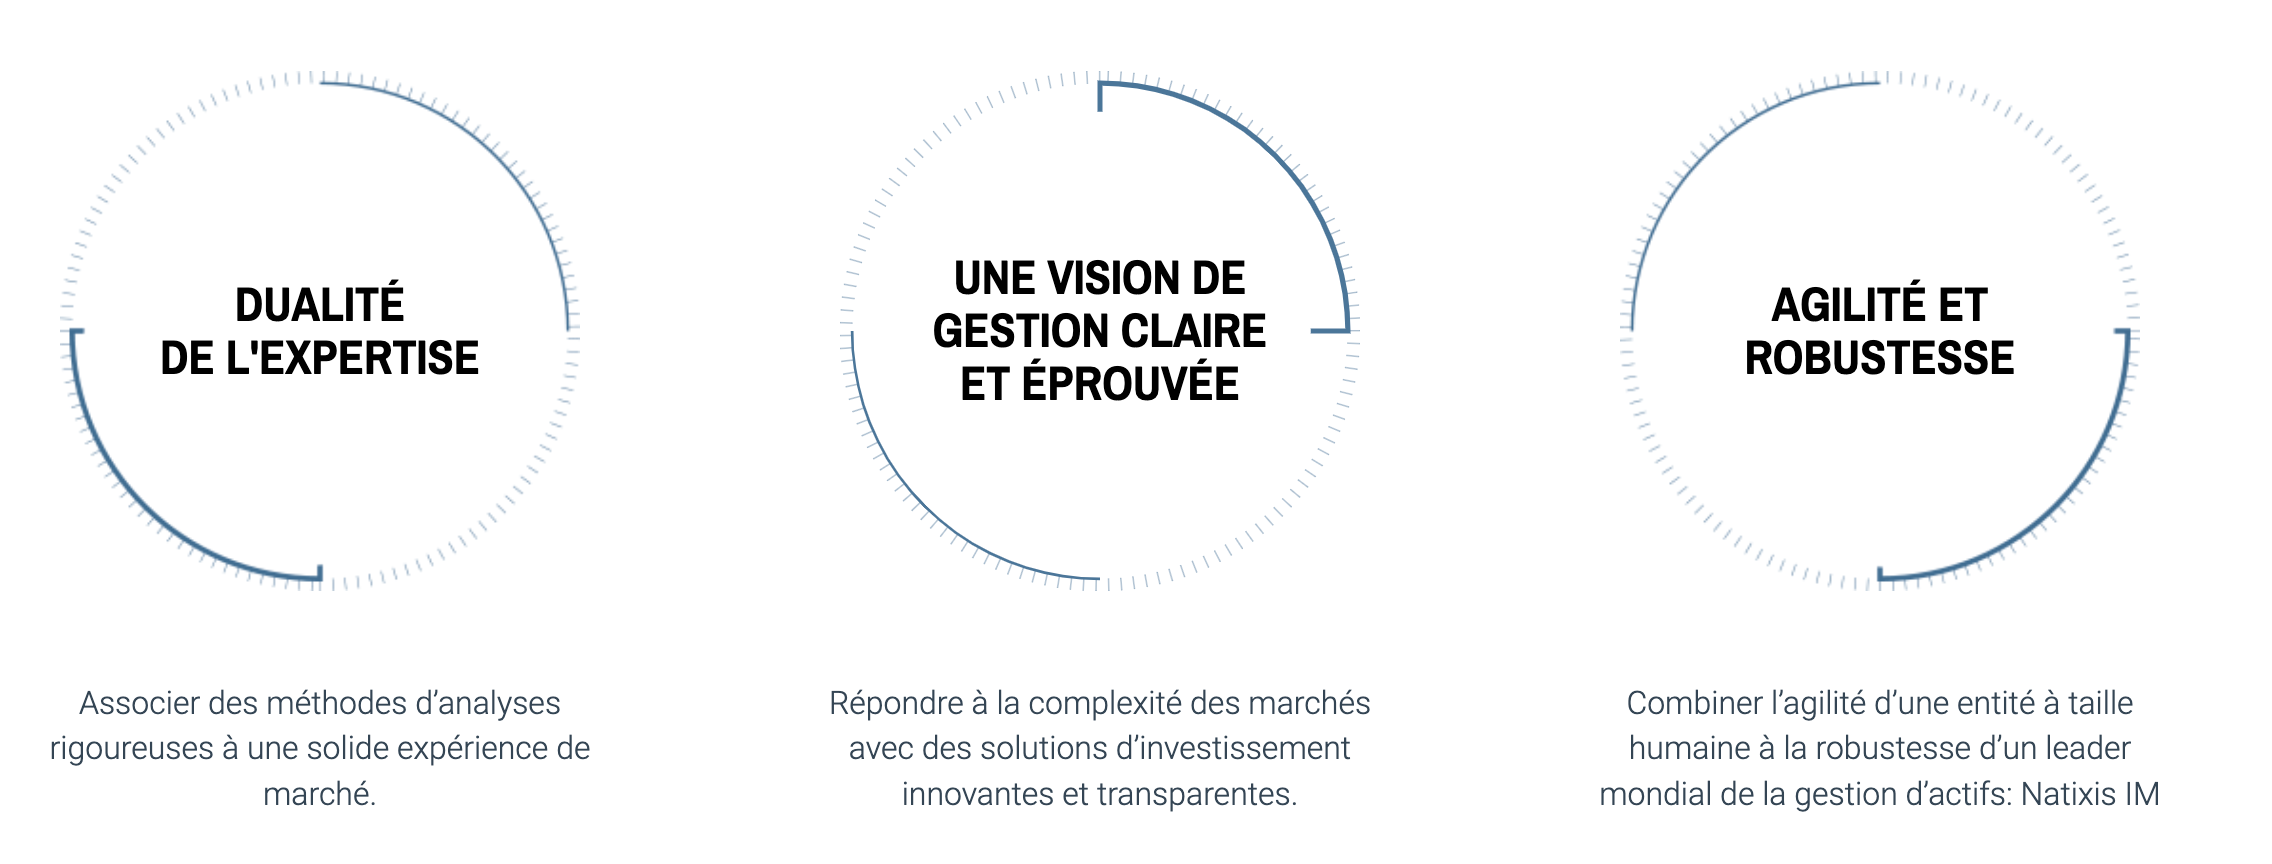
\includegraphics[width=\linewidth]{./img/intro/seeyond_objectifs}
\end{figure}

Seeyond est un spécialiste de la gestion quantitative active. A travers une approche intégrant une dimension humaine à la rigueur de processus d’investissement quantitatifs, les stratégies de gestion de Seeyond recherchent une rémunération optimale du risque, et ce sur trois expertises cœur : 
\begin{itemize}
\item Gestion Actions : Une expertise dont l’objectif est de transformer les primes de risque* actions et les anomalies de marché en source de performance.
\item Gestion Multi-asset : Une allocation active et flexible entre différentes classes d’actifs combinant convictions des gérants et indicateurs objectifs d’analyse de marché.
\item Gestion Volatilité \& Overlay : Des stratégies de gestion dédiées à la volatilité en tant que classe d’actifs.
\end{itemize}

Ces stratégies bénéficient de la longue expérience sur les marchés financiers et en analyse quantitative des professionnels de Seeyond.

\begin{figure}[h!]
  \caption{Titre de la figure (source : \cite{arrow48})}
  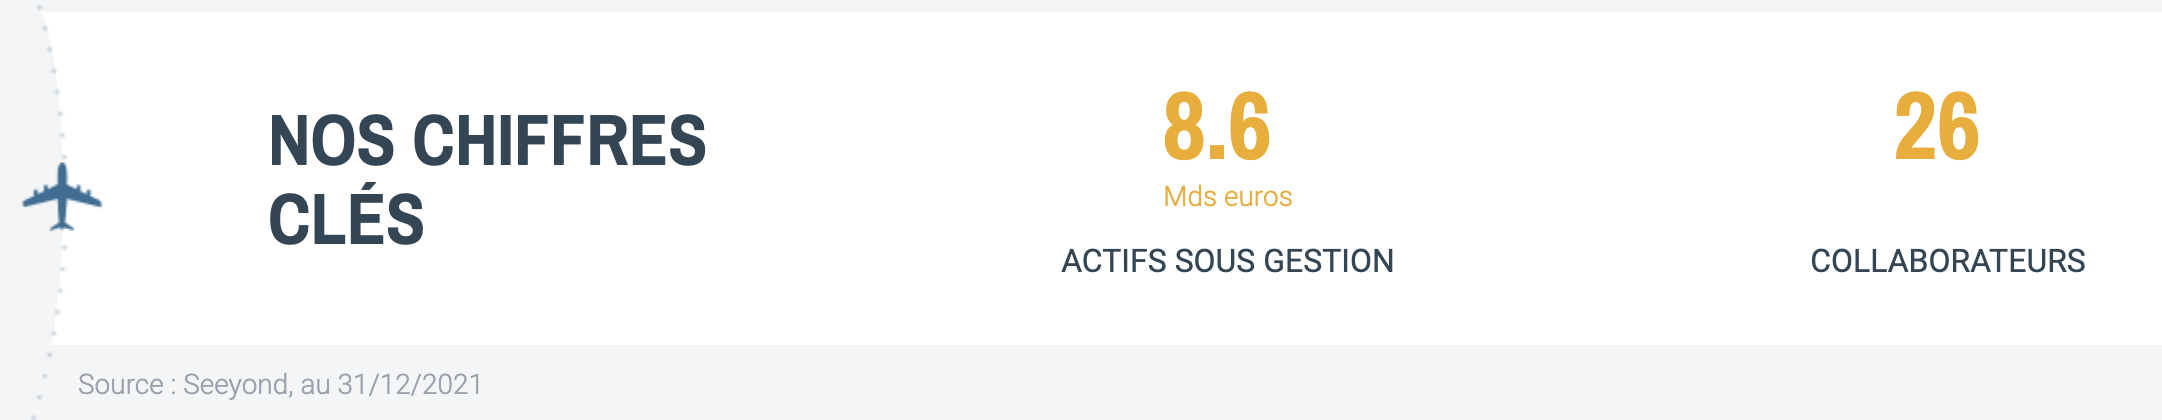
\includegraphics[width=\linewidth]{./img/intro/seeyond_kpi}
\end{figure}


En 2012, les équipes dédiées à la gestion quantitative* active du groupe Natixis Investment Managers, l’un des leaders mondiaux de la gestion d’actifs, ont été regroupées au sein d’une division de gestion dédiée avec une marque propre : Seeyond.
\\
En 2018, forte de son développement en tant que division de gestion, Seeyond est devenue une société indépendante et filiale à part entière du groupe Natixis IM.

\begin{figure}[h!]
  \caption{Titre de la figure (source : )}
  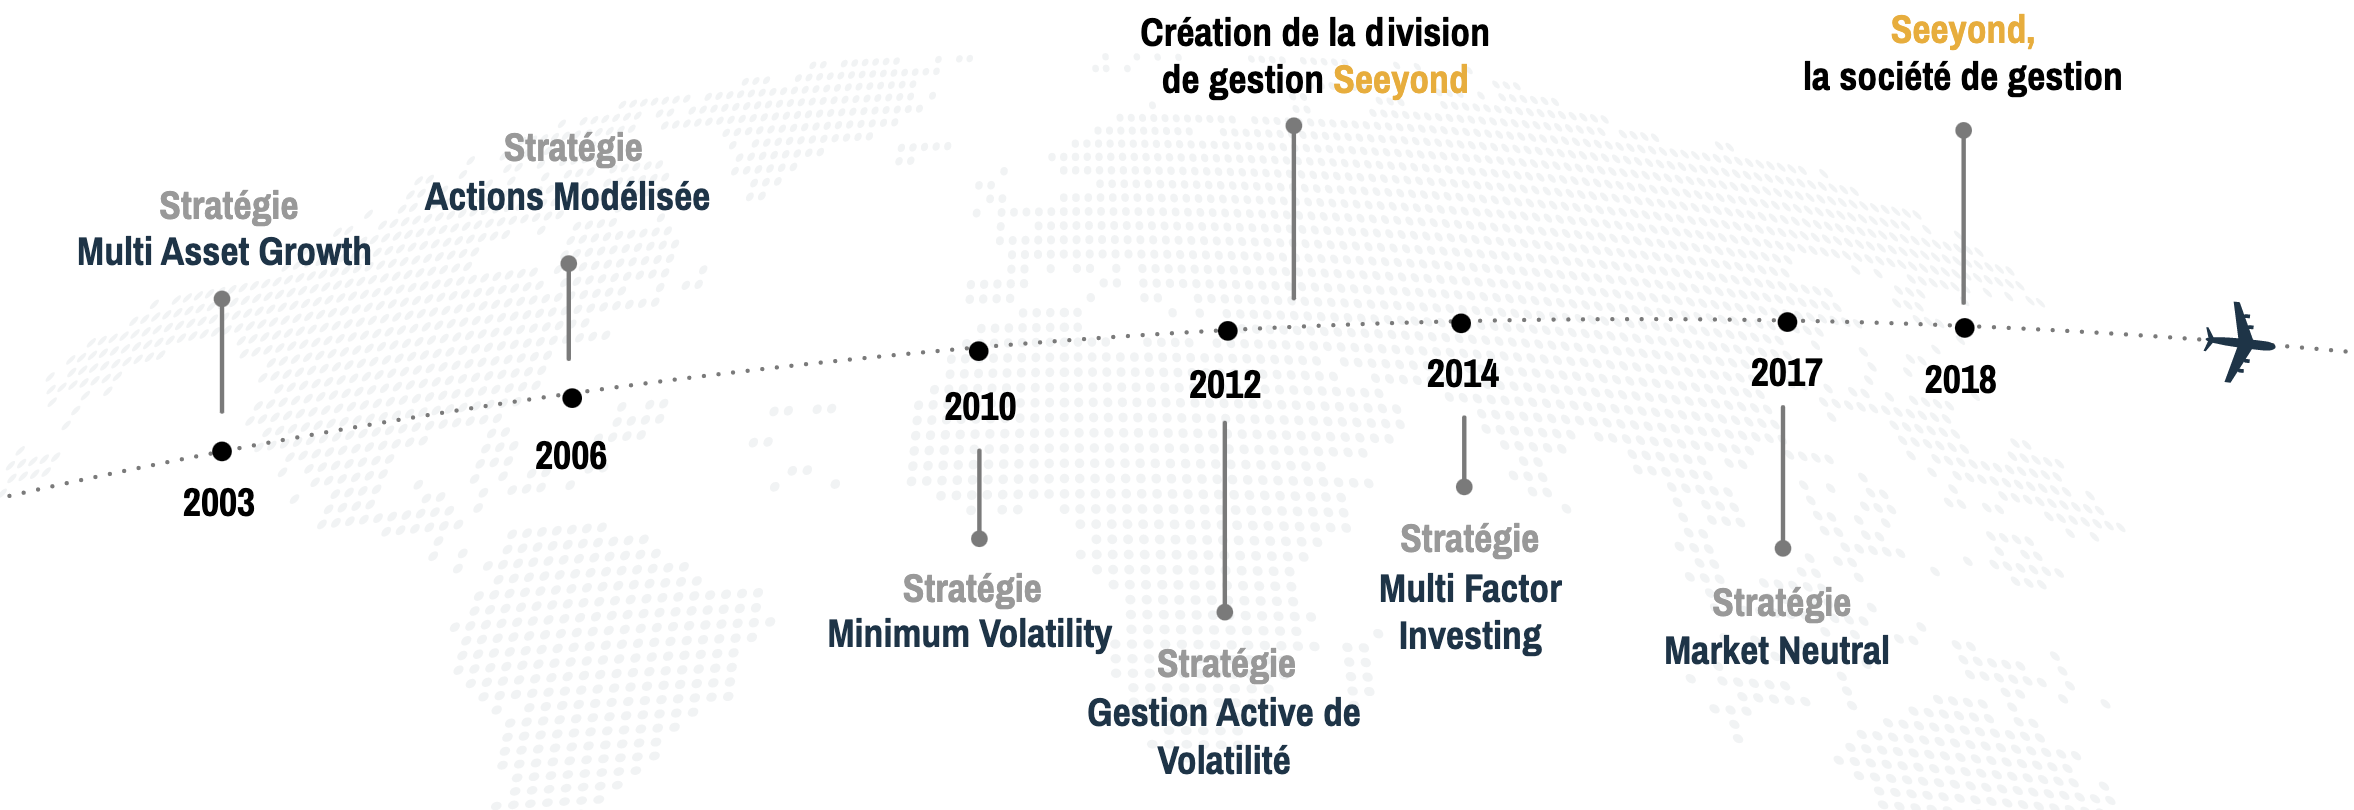
\includegraphics[width=\linewidth]{./img/intro/seeyond_hist}
\end{figure}



\newpage



\section*{Mon équipe}
%    \addcontentsline{toc}{section}{Mon équipe} 
Je fais parti de l'équipe RAD pour Rapid Application Development. La mission de cette équipe est de proposer un développement de proximité avec les différents services de Seeyond. Nous intervenons à la fois pour maintenir le système existant et pour développer de nouvelles fonctionnalités ou de nouveaux outils. Pour cela nous sommes en contact quotidiennement avec les membres de ces équipes afin de comprendre et répondre à leurs besoins.
\\
\\
Nous intervenons sur l'ensemble de la chaîne Front to Back, notamment avec la gestion, la recherche et la finance. Nous sommes amené à travailler sur des problématiques de gestion de portfeuille, de couvertures des risques, de suivie de transactions et bien d'autres.
\\
\\
Une de nos missions actuelle est de migrer les outils existant en VBA vers Python. L'intérêt de cette migration est de moderniser les outils en facilitant leurs développements futurs et en améliorant leur performance d'éxécution. De plus, nous profitons de cette migration pour regrouper l'ensemble des outils dans Enigma, une application web commune à toutes les équipes.

\newpage



\section*{Ma mission}
%\addcontentsline{toc}{section}{Ma mission} 
\subsection*{Mes réalisations}
\addcontentsline{toc}{subsection}{Mes réalisations} 
J'ai travaillé avec l'équipe RAD sur la maintenance des outils existants et sur de nouveaux développements. En particulier sur la migration d'outil VBA en python et sur leur intégration dans l'application Enigma.
\\
\\
J'ai par exemple travaillé sur un outil de calcul des commissions de sur-performance de certains fonds. En effet, Seeyond est un asset-manager qui se rémunère grâce aux frais récupérés des fonds sous-gestion. Des commissions de sur-performance s'appliquent sur certains portfeuilles Lorsqu'ils "battent" un indice qui sert de benchmark/comparatif. 
\\
Comme il peut s'agir de sommes importantes, ce calcul est réglementé. On le fait en interne et on doit le comparer à celui fait par un organisme externe. Il doit y avoir une trace/un historique de ces calculs.
\\
\\
J'ai aussi travaillé sur un outil permettant de générer divers graphiques sur les différents fonds gérés par Seeyond comme le drawdown sur une période donnée, la performance du fond par rapport à son benchmark, ... Cet outil est utilisé par les commerciaux afin de générer leurs présentations clients.

\subsection*{Problématique en lien avec l'équipe RAD}
%\addcontentsline{toc}{subsection}{Problématique en lien avec l'équipe RAD} 
La problématique de mon mémoire est d'utiliser l'algorithme UMAP (\textcolor{red}{le mot complet}) sur un jeu de données contenant diverses caractéristiques sur des actions depuis 1997.
\\
L'objectif est double, premièrement il faut essayer de repérer les caractéristiques des titres à faible volatilité qui sont susceptibles de voir leur volatilité augmenter à une horizon proche. Ensuite il faut améliorer la visualisation de ces données.
\\
\\
L'intérêt pour la gestion action est de pouvoir repérer les titres stables, pour assurer une certaine sécurité notamment en période de "crises".
\\
Il s'agit d'un problématique de recherche. ( Selon le résultat il n'y aura pas nécessairement la création d'un nouvel outil. ) 